\chapter{System Evaluation}
This chapter evaluates the system, analysing the various aspects of the project 
to ensure the requirements of the project were met and discusses the various 
types of testing that was performed throughout the software development cycle to
ensure each of the requirements was met and the software was of high quality. 

\section{Overview}
The system was designed and developed using the Test Driven Development (TDD) 
methodology. As each unit of code was written and before each new component was 
integrated into the system, appropriate tests were carried out and adjusted if 
needed. Because of this, a lot of bugs were caught early on, allowing them to be
fixed with minimal disruption to the system as a whole. This also allowed the 
system to be redesigned early on when necessary.

\par
\bigskip
The types of testing carried out were as follows:

\begin{itemize}
    \item End-to-End Testing
    \item Exploratory Testing
    \item Functional Testing
    \item Graphical User Interface (GUI) Testing
    \item Integration Testing
    \item Unit Testing
    \item System Testing
\end{itemize}

\section{End-to-End Testing}
\begin{center}
    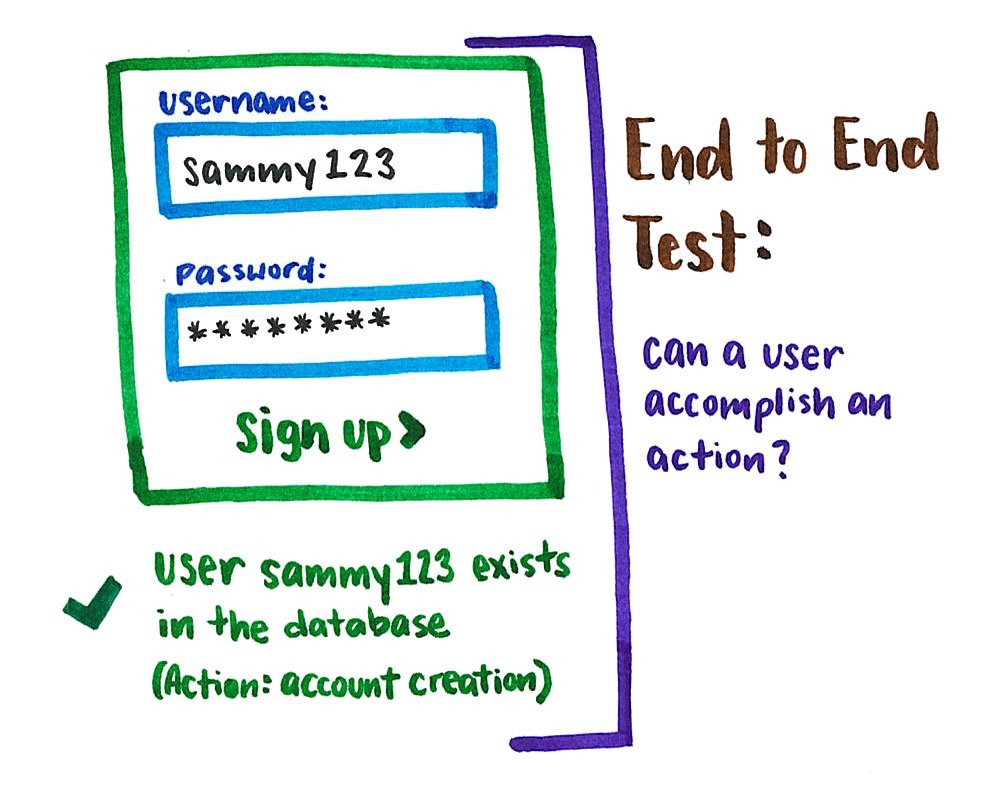
\includegraphics[width=6cm,height=10cm,keepaspectratio]{images/e2e_1}
    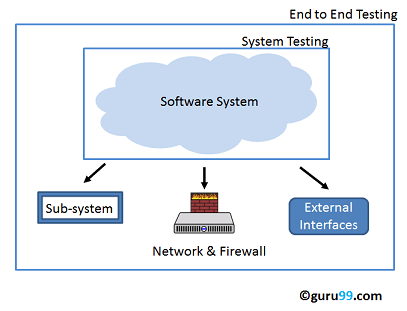
\includegraphics[width=6cm,height=10cm,keepaspectratio]{images/e2e_2}
\end{center}

End-to-end testing is a technique used to test whether the flow of an 
application right from start to finish is behaving as expected. The purpose of 
performing end-to-end testing is to identify system dependencies and to ensure
that the data integrity is maintained between various system components and 
systems.
\par
\bigskip
The entire application is tested for critical functionalities such as 
communicating with the other systems, interfaces, database, network, and other 
applications. This type of testing was carried out at the end, when all features were fully implemented. To perform 'test cases', the system was used in a way that a user would typically use the system. All features were tested to see if the appropriate behaviour happened, such as visualizing an algorithm, registering for an account, logging into an account, recording a sort, uploading a sort, and viewing past sorts.

\section{Exploratory Testing}
\begin{center}
    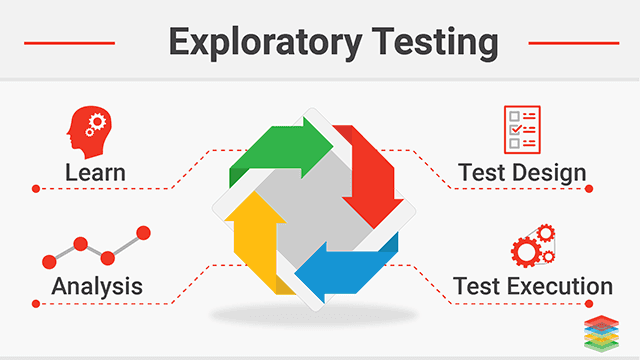
\includegraphics[width=12cm,height=10cm,keepaspectratio]{images/xenonstack-what-is-exploratory-testing}
\end{center}
Exploratory testing is a technique or a method whose aim is to discover the
flaws during the process of software development. Exploratory Testing is widely used in Agile models and is all about discovery, investigation, and learning. It emphasizes personal freedom and responsibility of the individual tester.

\par
\bigskip

This technique of testing is concerned about the qualitative assurance of the 
software. It is used to discover the anonymous issues during the process of 
development of software. Exploratory testing was carried out throughout development and helped prevent massive system flaws from remaining in the application and causing other bugs and/or having to fix these issues down the line, where it mightn't be possible to fix them or having to perform a complete overhaul of the system. One such flaw was in regards to an early design. Initially, there would be a 'master' navigation bar, with each of the application's pages appearing and being able to be navigated to from here. This caused the visualization aspect to not work properly, as the user would not be able to select an algorithm to visualize. This resulted in the system being redesigned to what it is now.

\section{Functional Testing}
\begin{center}
    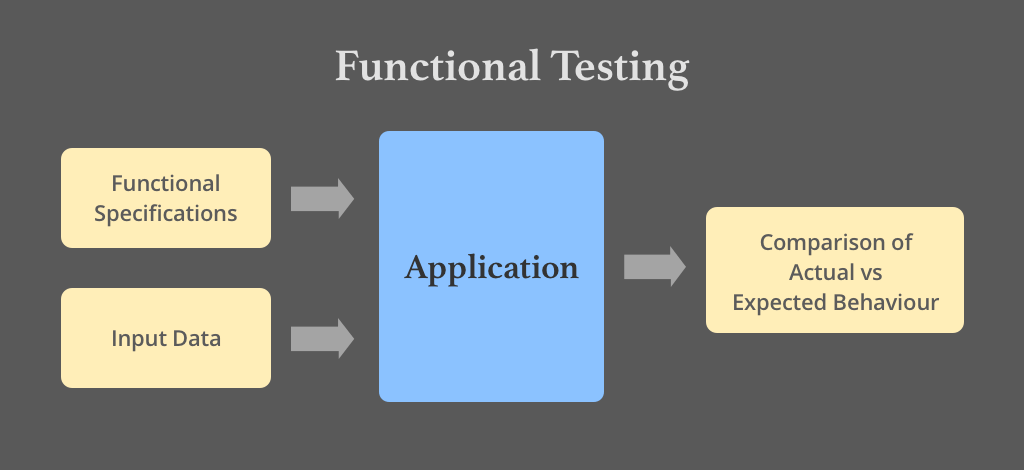
\includegraphics[width=12cm,height=10cm,keepaspectratio]{images/Functional-Testing-feature-image}
\end{center}
Functional Testing is a type of software testing whereby the system is tested 
against the functional requirements/specifications.
\par
\bigskip
Functions (or features) are tested by feeding them input and examining the 
output. Functional testing ensures that the requirements are properly satisfied 
by the application. This type of testing is not concerned with how processing 
occurs, but rather, with the results of processing. It simulates actual system 
usage but does not make any system structure assumptions.
\par
\bigskip
During functional testing, Black Box Testing technique is used in which the 
internal logic of the system being tested is not known to the tester.

\section{Graphical User Interface (GUI) Testing}
\begin{center}
    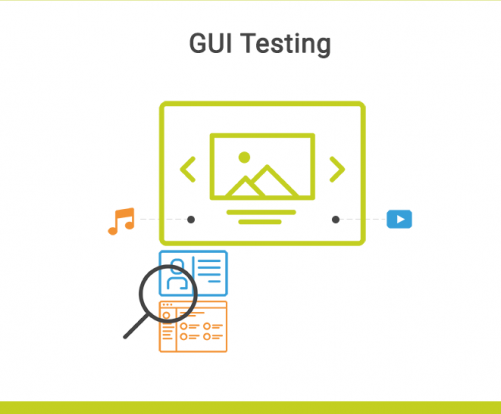
\includegraphics[width=12cm,height=10cm,keepaspectratio]{images/gui_testing}
\end{center}
Graphical User Interface (GUI) Testing is a software testing type that checks
the Graphical User Interface of the application under test. GUI testing involves
checking the screens with the controls like menus, buttons, icons, and all types
of bars - toolbar, menu bar, dialog boxes, and windows, etc. The purpose of GUI 
Testing is to ensure UI functionality works as per the specification. 
\par
\bigskip
This type of testing, like exploratory testing, was carried out in conjunction with development and as such, aided in discovering bugs with the system. As discussed above, the system needed to be redesigned due a bug discovered, which GUI testing aided in as it was discovered in a previous design that the user was not able to visualize an algorithm due to an unresponsive GUI.

\section{Integration Testing}
\begin{center}
    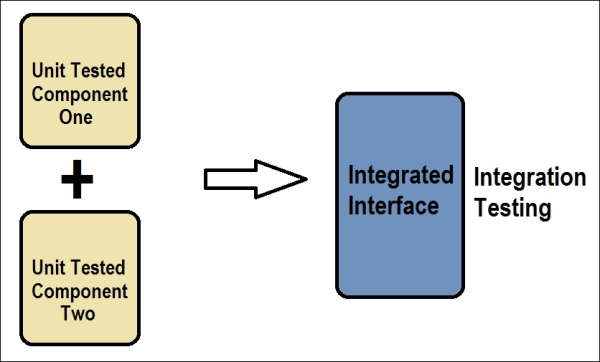
\includegraphics[width=12cm,height=10cm,keepaspectratio]{images/integration}
\end{center}
Integration testing (sometimes called integration and testing, abbreviated I&T) 
is the phase in software testing in which individual software modules are 
combined and tested as a group. Integration testing is conducted to evaluate the
compliance of a system or component with specified functional requirements.
\par
\bigskip
Integration testing was carried out throughout development and was integral in ensuring components worked with already integrated components without breaking the system. When a new component was added to the application, the entire application was tested in full before committing the changes to GitHub to make sure the new component didn't negatively affect or break the application. 

\section{Unit Testing}
\begin{center}
    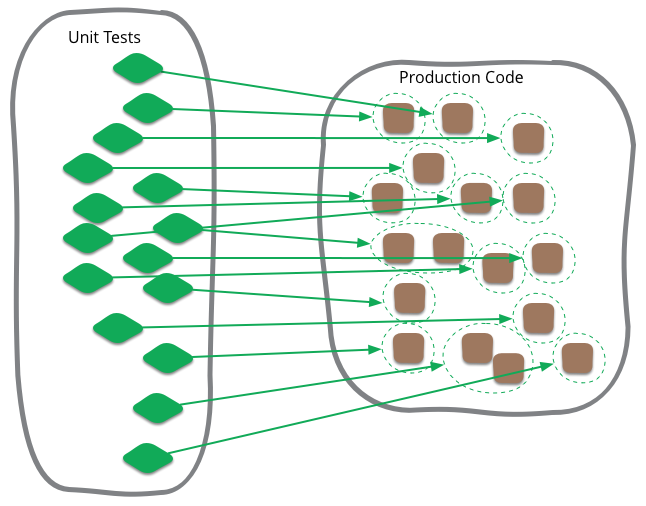
\includegraphics[width=12cm,height=8cm,keepaspectratio]{images/unit}
\end{center}
Unit Testing is a level of software testing where individual units/components
of a software are tested. The purpose is to validate that each unit of the
software performs as designed. A unit is the smallest testable part of any 
software. It usually has one or a few inputs and usually a single output.
\par
\bigskip
Unit testing was carried out on individual components before they were integrated into the system. Several different pieces of software were used to help test the application.

\subsection{Postman}
\begin{center}
    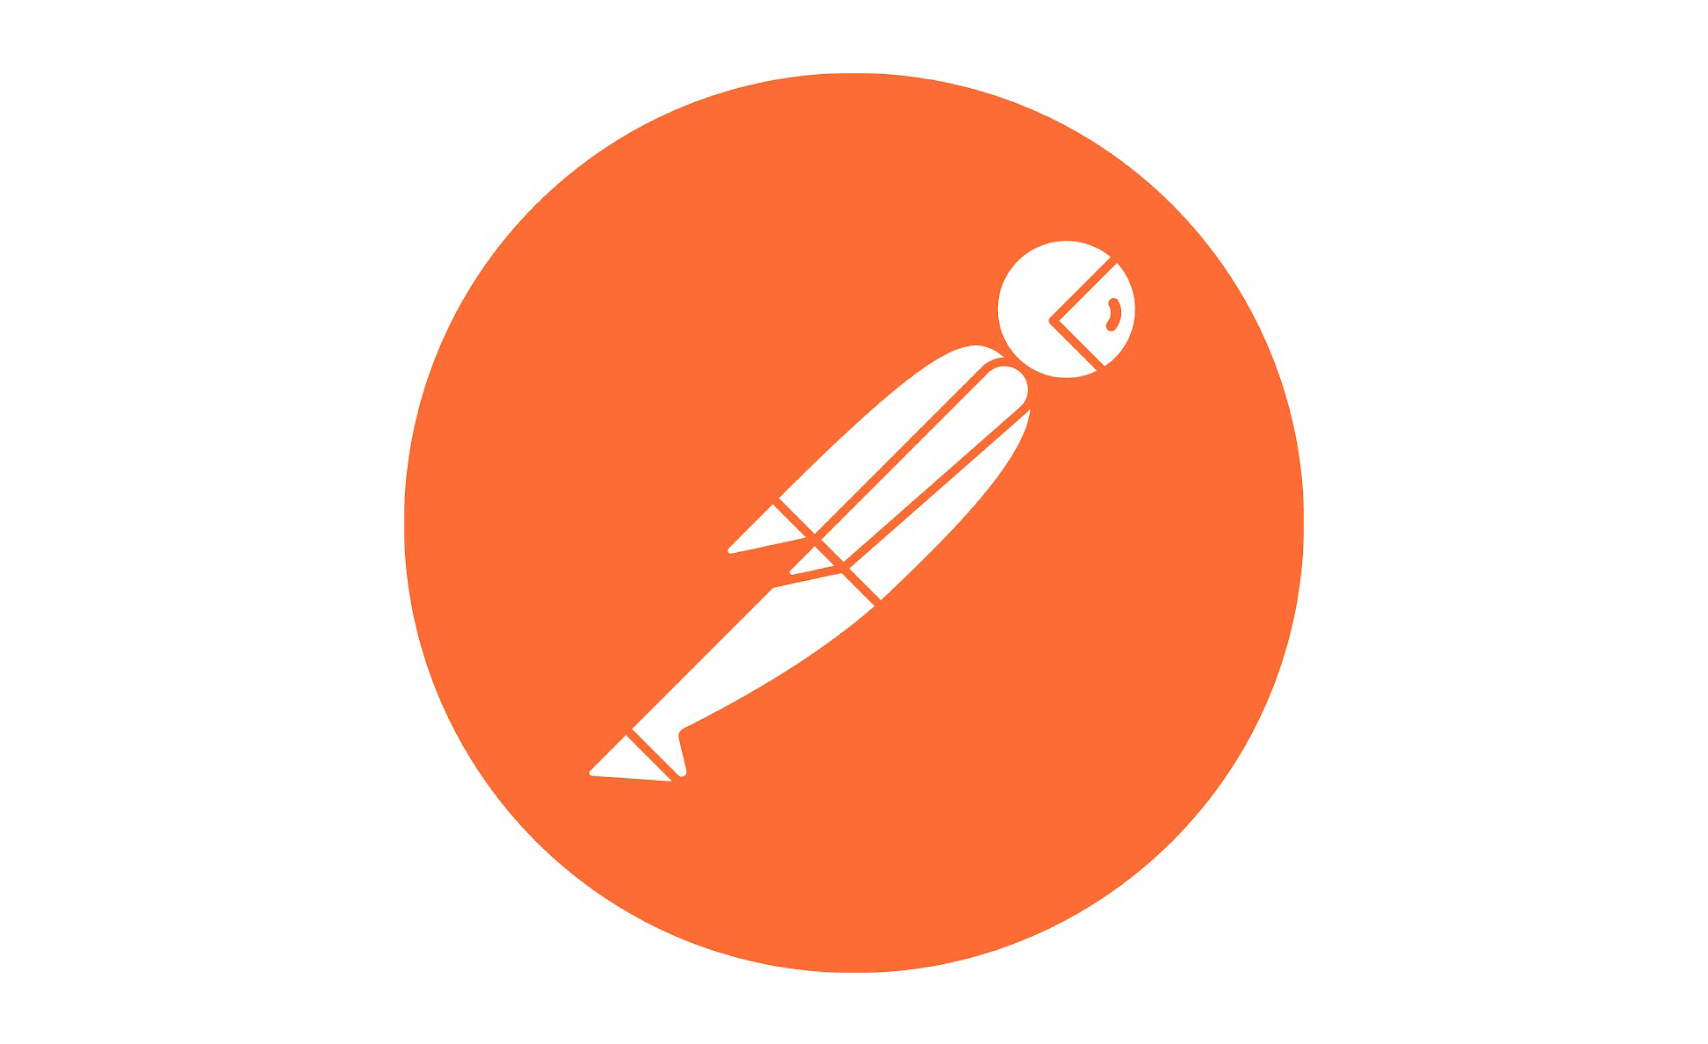
\includegraphics[width=12cm,height=4cm,keepaspectratio]{images/postman}
\end{center}
To test the user authentication aspect of the application, Postman was used to test requests made to the database to see if a user could successfully register for an account and log into an account. Requests could be made to the database via the Flask Server (hosted on PythonAnywhere), which would then return a response.

\subsubsection{Register}
\begin{center}
    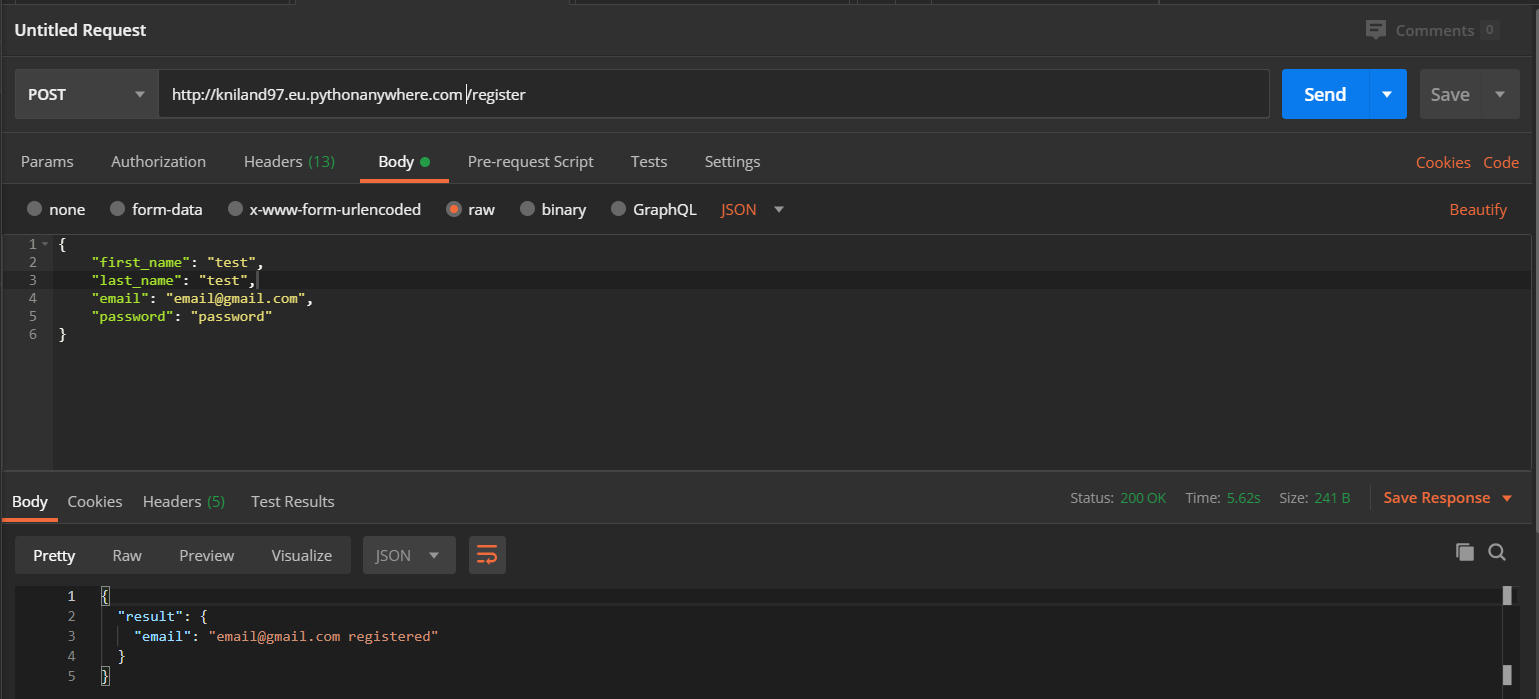
\includegraphics[width=12cm,height=4cm,keepaspectratio]{images/postman_register}
\end{center}
Using the POST method, a request is made to see if a user with the above details is able to successfully register an account with the application.

\subsubsection{Login}
\begin{center}
    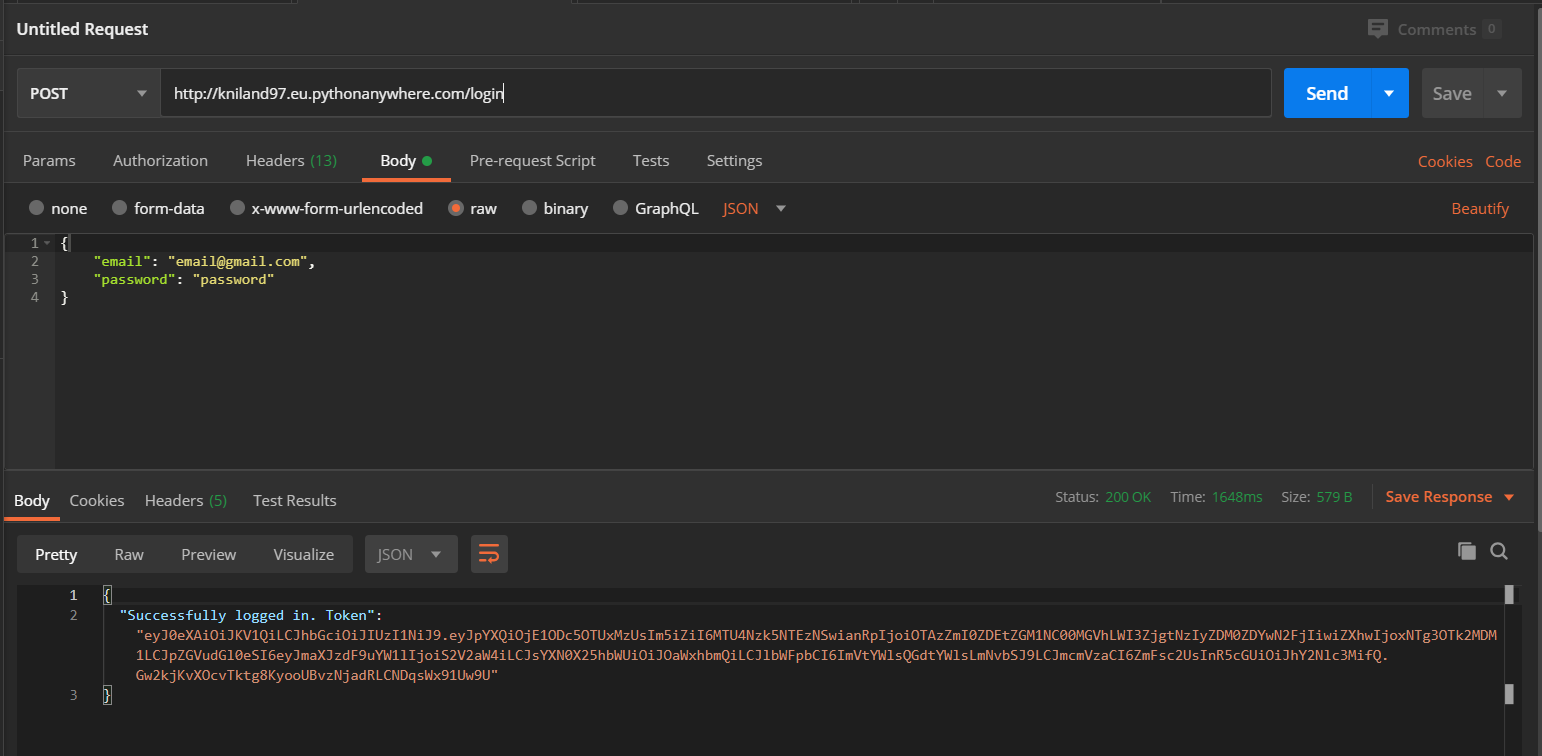
\includegraphics[width=12cm,height=4cm,keepaspectratio]{images/postman_login}
\end{center}
Using the POST method, a request is made to see if a user with the above details is able to successfully login to the application.

\subsection{Sorting Algorithms}
Before each sorting algorithm was implemented and added into the application, they were first written and tested on sample inputs and arrays.

\section{System Testing}
\begin{center}
    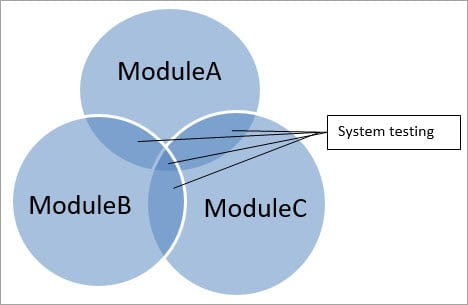
\includegraphics[width=12cm,height=10cm,keepaspectratio]{images/system-testing-example}
\end{center}
System Testing is a level of testing that validates the complete and fully
integrated software product. The purpose of a system test is to evaluate the 
end-to-end system specifications. Usually, the software is only one element of a
larger computer-based system. Ultimately, the software is interfaced with other 
software/hardware systems.

\subsection{Selenium}
\begin{center}
    
\includegraphics[scale=0.15,keepaspectratio]{images/selenium_logo_large}
\end{center}
Selenium was used to test the system as a whole. Selenium is a portable framework for testing web applications. It also provides a test domain-specific language (Selenese) to write tests in a number of popular programming languages, including C#, Groovy, Java, Perl, PHP, Python, Ruby and Scala. The tests can then run against most modern web browsers.

\begin{center}
    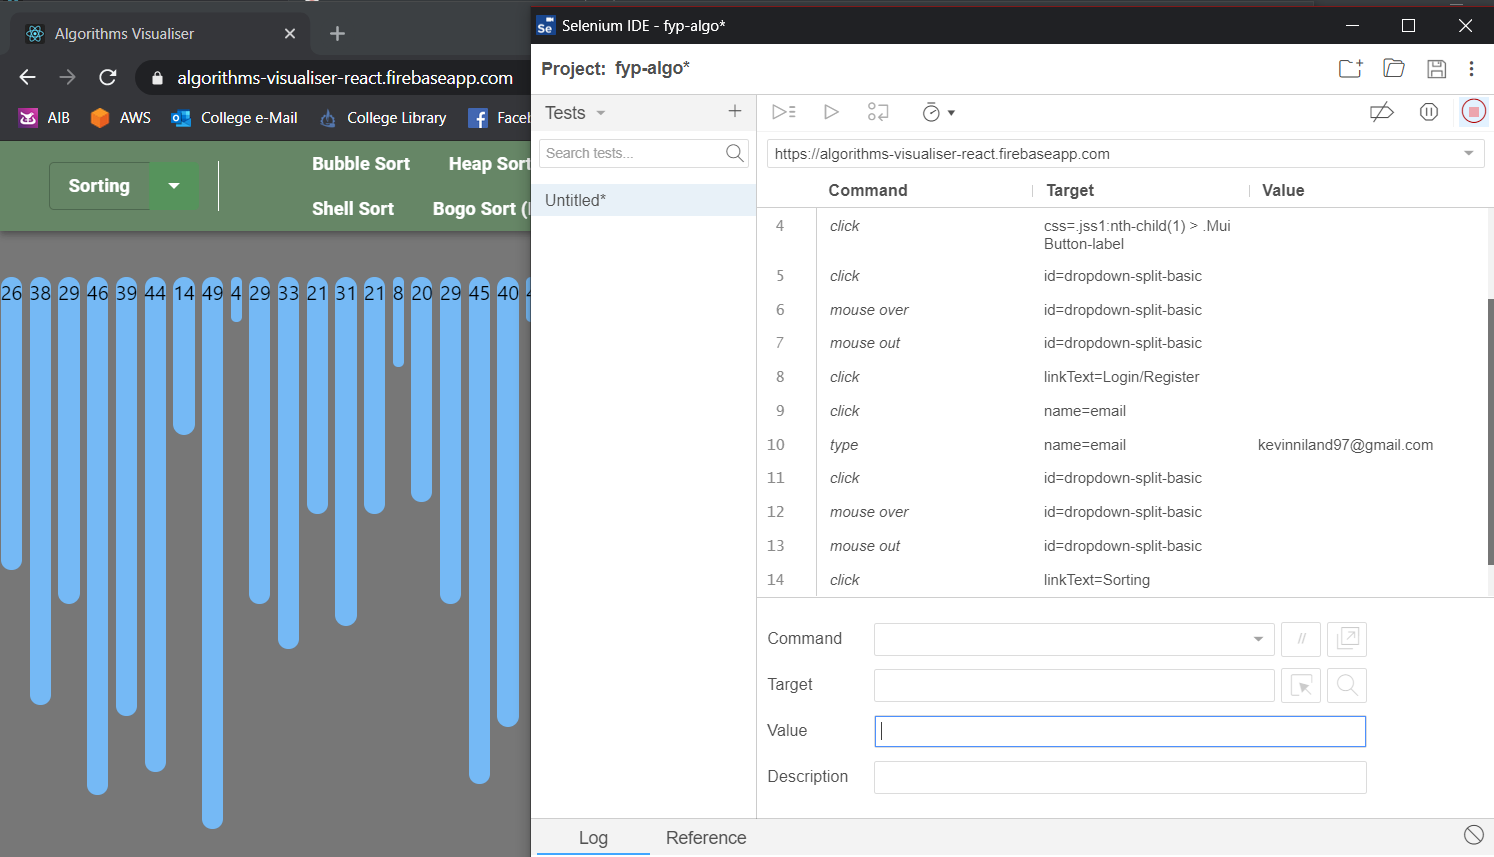
\includegraphics[width=12cm,height=6cm,keepaspectratio]{images/selenium}
\end{center}
Selenium provides the option to record, edit, and debugging of functional tests. As can be seen, Selenium allows one to test various functionality of a web application such as button clicks, mouse over, mouse out, typing, etc. This functionality can be tested on the fly (as in, you can specify the URL of the web application and test the functionality of the web application yourself) or define a test case and then run it (such as clicking and verifying a specific button or entering text into a textbox).